\documentclass[11pt,xcolor=svgnames]{beamer}
\usepackage{dsfont,natbib,setspace,changepage,multirow}
\mode<presentation>

% replaces beamer foot with simple page number
\setbeamertemplate{navigation symbols}{}
%\setbeamerfont{frametitle}{series=\bfseries}
\setbeamercolor{frametitle}{fg=Black}

\setbeamertemplate{footline}{
   \raisebox{5pt}{\makebox[\paperwidth]{\hfill\makebox[20pt]{\color{gray}\scriptsize\insertframenumber}}}}

\graphicspath{{/Users/mtaddy/Dropbox/inputs/}}
\usepackage{algorithm}
\usepackage{algorithmic}

% colors
\newcommand{\theme}{\color{Maroon}}
\newcommand{\bk}{\color{black}}
\newcommand{\rd}{\color{DarkRed}}
\newcommand{\fg}{\color{ForestGreen}}
\newcommand{\bl}{\color{blue}}
\newcommand{\gr}{\color{black!50}}
\newcommand{\sg}{\color{DarkSlateGray}}
\newcommand{\nv}{\color{Navy}}
\setbeamercolor{itemize item}{fg=gray}

% common math markups
\newcommand{\bs}[1]{\boldsymbol{#1}}
\newcommand{\mc}[1]{\mathcal{#1}}
\newcommand{\mr}[1]{\mathrm{#1}}
\newcommand{\bm}[1]{\mathbf{#1}}
\newcommand{\ds}[1]{\mathds{#1}}
\newcommand{\indep}{\perp\!\!\!\perp}
\def\plus{\texttt{+}}
\def\minus{\texttt{-}}

% spacing and style shorthand
\setstretch{1.1}

\begin{document}

\setcounter{page}{0}
{ \usebackgroundtemplate{\includegraphics[height=\paperheight]{phoenix}}
\begin{frame}[plain]
\begin{center}


{\bf \Large Big Data and Bayesian Nonparametrics}

\vskip 2cm
Matt Taddy,  Chicago Booth


\vskip .25cm
{\texttt{faculty.chicagobooth.edu/matt.taddy/research}}

\end{center}
\end{frame} }

\begin{frame}


{\bf Big Data}

\vskip .5cm
{The sample sizes are enormous. {\gr 200\texttt{+} million obs}}

{The data are super weird.  {\gr density spikes, obese tails}}

\vskip .25cm
`Big' and `Strange' beg for nonparametrics.

\vskip .5cm
In usual BNP you {\it model} a complex generative process with flexible priors, then apply that model directly in prediction and inference.
\[
\text{e.g.,~~~}y = f(\bm{x}) + \epsilon,~~\text{or~even~just}~~f(y|\bm{x})
\]
However averaging over all of the nuisance parameters we introduce to be `flexible' is a hard computational problem.

\vskip .5cm
\hfill {\theme Can we do scalable BNP?}

\end{frame}

\begin{frame}

Frequentists are great at finding simple procedures {\gr\small (e.g. $[\bm{X}'\bm{X}]^{-1}\bm{X}'y$)\!} and  showing that they will `work' regardless of the true DGP.

\hfill{\gr \small (DGP = Data Generating Process)~~~~~~~}

\vskip .5cm
This is classical `distribution free' nonparametrics.

\vskip .15cm
1: Find some statistic that is useful regardless of DGP.

\vskip .15cm
2: Derive the distribution for this stat under minimal assumptions.

\vskip .5cm
Practitioners apply the simple stat and feel happy that it will work.

% {\gr No need to re-model the underlying DGP each time, and you \\don't need to have a PhD in Bayesian Statistics to apply the ideas.}

\vskip .5cm\hfill
{\theme Can we Bayesians provide something like this?}

\end{frame}

\begin{frame}

{\bf A flexible model for the DGP}
\begin{equation*}
g(\bm{z}) = \frac{1}{|\bs{\theta}|}\sum_{l=1}^L \theta_l \ds{1}{[\bm{z} =
\bs{\zeta}_l]}, ~~~ \theta_l/|\bs{\theta}| \stackrel{iid}{\sim} \mr{Dir}(a)\end{equation*}

\vskip .25cm
After observing $\bm{Z} = \{\bm{z}_1 \ldots \bm{z}_n\}$, posterior has $\theta_l \sim \mr{Exp}(a\!+\!\ds{1}_{\bs{\zeta}_l \in \bm{Z}})$. {\gr (say every $\bm{z}_i = [\bm{x}_i,y_i]$ is unique)}.

\vskip .5cm
$a \to 0$ leads to $\mr{p}(\theta_l = 0) = 1$ for $\bs{\zeta}_l \notin \bm{Z}$.
\[
\Rightarrow g(\bm{z}\mid\bm{Z}) = \tfrac{1}{|\bs{\theta}|}
\sum_{l=1}^L \theta_l \ds{1}{[\bm{z} =
\bm{z}_l]},~~~\theta_i \sim \mr{Exp}(1)
\]

\hfill
{This is just the Bayesian bootstrap.}

\hfill {\gr Ferguson 1973, Rubin 1981}

\end{frame}

\begin{frame}

{\bf {\gr Example: } Ordinary Least Squares}

\vskip .5cm
{\it Population} OLS is a posterior functional
\begin{equation*}
\bs{\beta} = (\bm{X}'\bs{\Theta}\bm{X})^{-1}  \bm{X}'\bs{\Theta}\bm{y}
\end{equation*}
where $\bs{\Theta} = \mr{diag}(\bs{\theta})$.  
{\theme This is a random variable. \gr (sample via BB)}

\vskip .5cm
Posterior moments for a first-order approx
\[
\bs{\tilde \beta} = [\bm{X}'\bm{X}]^{-1}\bm{X}'y + 
\nabla \bs{\beta}\big |_{\bs{\theta}=\bm{1}} (\bs{\theta} - \bm{1})
\]
e.g., $\mr{var}(\bs{\tilde \beta}) \approx (\bm{X}^{\prime}\bm{X})^{-1}\bm{X}^{\prime}\mr{diag}(\bm{e})^2\bm{X}^{\prime}(\bm{X}^{\prime}\bm{X})^{-1}$, where $e_i  = y_i - \bm{x}_i'\bs{\hat\beta}$.

\vskip .5cm{\gr \hfill
 See Lancaster 2003 or Poirier 2011.}

\end{frame}

\begin{frame}

{\bf User-Specific Behavior in Experiments}

\vskip .5cm
{eBay runs lots of experiments:} they make changes to the marketplace (website) for random samples of users.

\vskip .25cm
Every experiment has response $y$ {\gr (spend)} and treatment $d$ {\gr [0/1]}.

\vskip .05cm
In our illustrative example,
$d_i = 1$ for bigger pictures in my eBay.


\vskip .25cm
{\small $i\in{\sf c}: d_i=0$ \hspace{3.5cm} $i\in{\sf t}: d_i=1$}

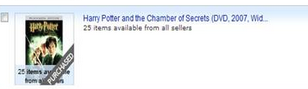
\includegraphics[scale=.5]{graphs/pottersmall}
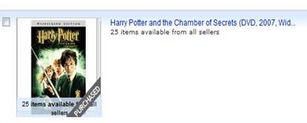
\includegraphics[scale=.5]{graphs/potterbig}


\vskip .5cm
We know $\bm{x}_i$ about user $i$: {\gr previous spend, last purchase date, items bought, sold, watched, bidded on, pages visited,  ...}

And every user responds diferently to the treatment.
\end{frame}

\begin{frame}



We can {\it index}  heterogeneity in treatment effect on $\bm{x}_i$ via
\[
\bs{\beta}_{\sf t} - \bs{\beta}_{\sf c} = (\bm{X}_{\sf t}'\bs{\Theta}_{\sf t}\bm{X}_{\sf t})^{-1}  \bm{X}_{\sf t}'\bs{\Theta}_{\sf t}\bm{y}_{\sf t} - (\bm{X}_{\sf c}'\bs{\Theta}_{\sf c}\bm{X}_{\sf c})^{-1}  \bm{X}_{\sf c}'\bs{\Theta}_{\sf c}\bm{y}_{\sf c} 
\] 

e.g., coefficient on purchase within last-year vs an intercept:

{\footnotesize\it
\gr million users:~~~~~~~~~~~~~~~7.45~~~~~~~~~~~~~~~~~~~~~~10.97~~~~~~~~~~~~~~~~~~~~~13.22}
\begin{center}
\vskip -.5cm
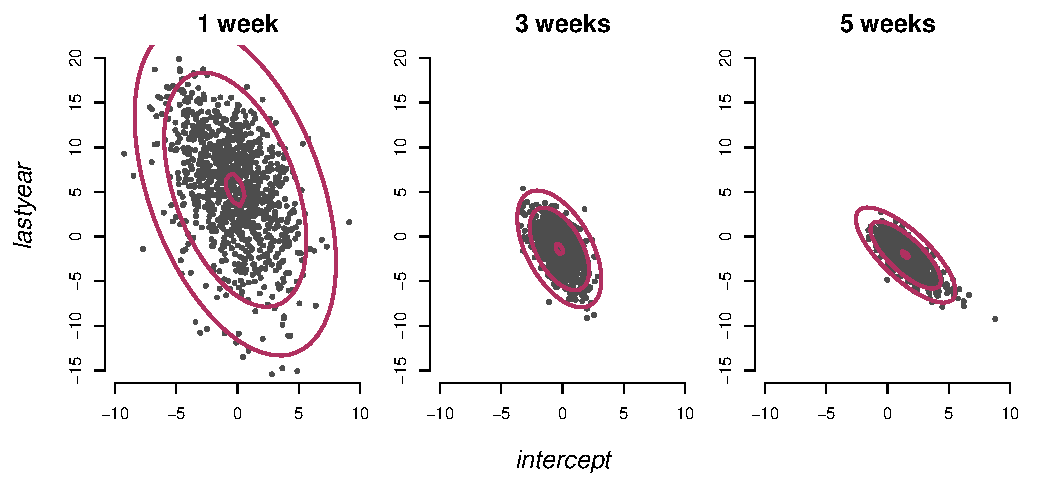
\includegraphics[width=.9\textwidth]{graphs/gammapost}
\end{center}

\vskip -.5cm
{\gr Sample is from posterior, contours are normal approximation.}

{This is a statistic we care about}, even if the truth is nonlinear.

\vskip -.5cm
\end{frame}

\begin{frame}


{\bf {\theme Example:} Decision Trees}

\vskip .5cm
Trees are great: nonlinearity, deep interactions, heteroskedasticity.

\begin{center}
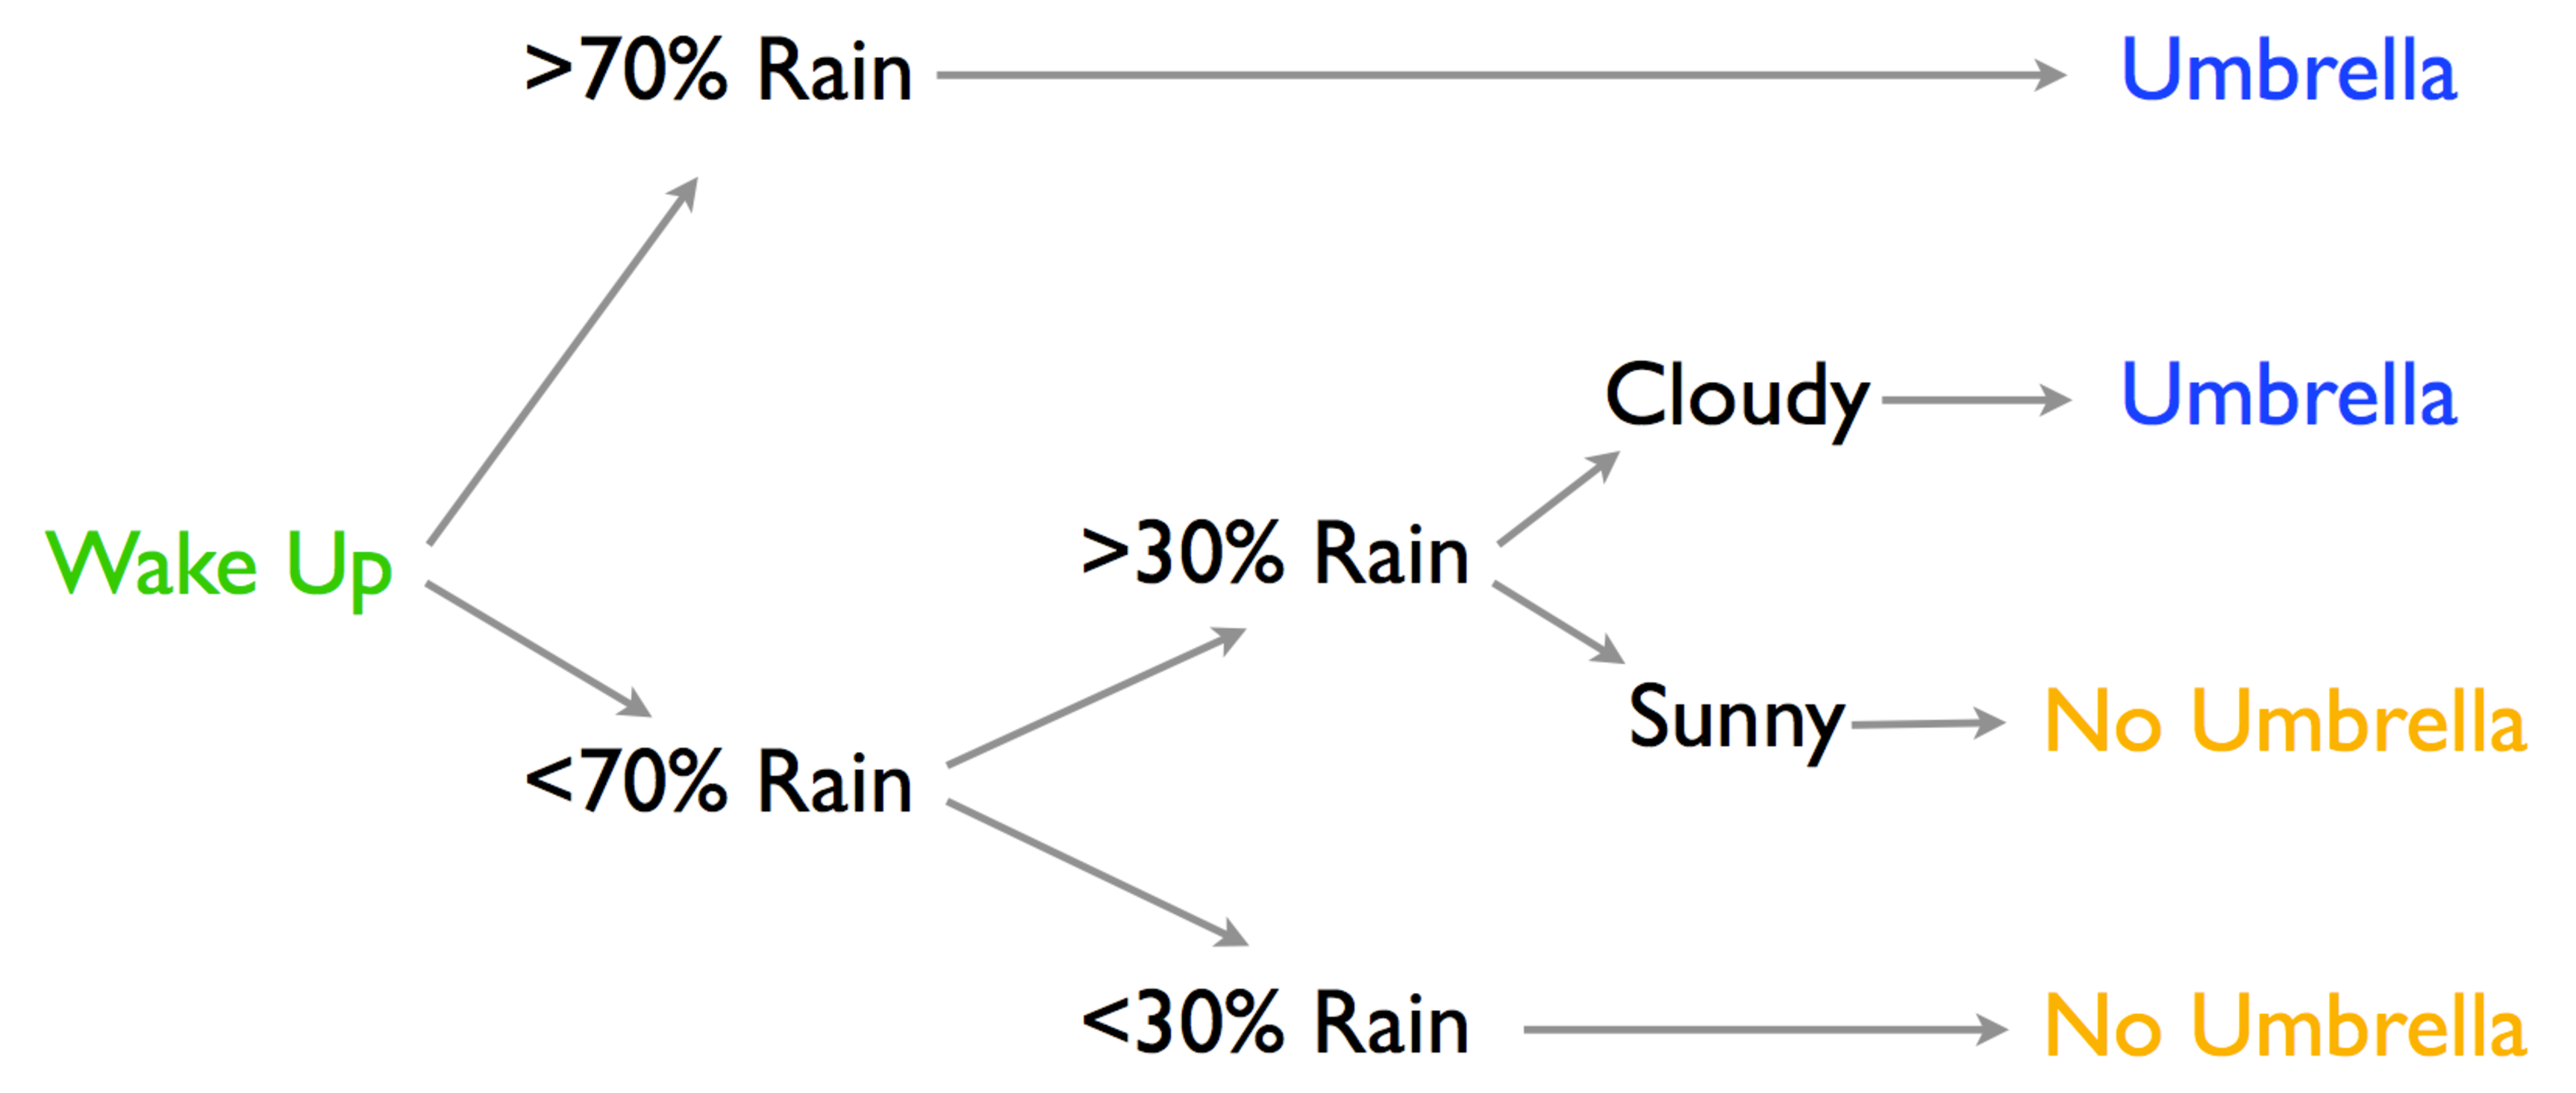
\includegraphics[width=4in]{../graphs/umbrella}
\end{center}

The `optimal' decision tree is a statistic we care about {\gr (s.w.c.a)}.


\end{frame}


\begin{frame}


{\bf {\theme CART:} greedy growing with optimal splits}

\vskip .5cm
Given node $\{\bm{x}_i,y_i\}_{i=1}^n$ and DGP weights $\bs{\theta}$,
find $x$ to minimize 
\begin{align*}
|\bs{\theta}|\sigma^2(x, \bs{\theta} ) &= \sum_{k \in \mathrm{left}(x)} \theta_k (y_k - \mu_{\mathrm{left}(x)})^2 \\&+ \sum_{k \in \mathrm{right}(x)} \theta_k (y_k - \mu_{\mathrm{right}(x)})^2
\end{align*}
for a regression tree.  Classification impurity can be Gini, etc.


\vskip .5cm
Population-CART might be a statistic we care about.


\vskip .1cm{\gr 
Or, in settings where greedy CART would do poorly (big $p$), \\a randomized splitting algorithm might be a better s.w.c.a.}



\end{frame}


\begin{frame}[fragile]

{\bf \theme Bayesian Forests: \bk a posterior for CART trees}

\vskip .25cm
For $b=1 \dots B$: \\
   ~~~~~~~~~~$\bullet$ draw $\boldsymbol{\theta}^b \stackrel{iid}{\sim} \mathrm{Exp}(\mathbf{1})$
   \\
   ~~~~~~~~~~$\bullet$ run weighted-sample CART to get $\mathcal{T}_b = \mathcal{T}(\boldsymbol{\theta}^b)$
 
\vskip .5cm\small 
~~~~~~~~~~~~~~~~~~~~~{\it one tree~~~~~~~~~~~~~~~~~~~~~~~~~~~~~~~~~~posterior mean}\\

\includegraphics[height=1.75in]{../../bayesian-forest/graphs/MCtreedraw}   
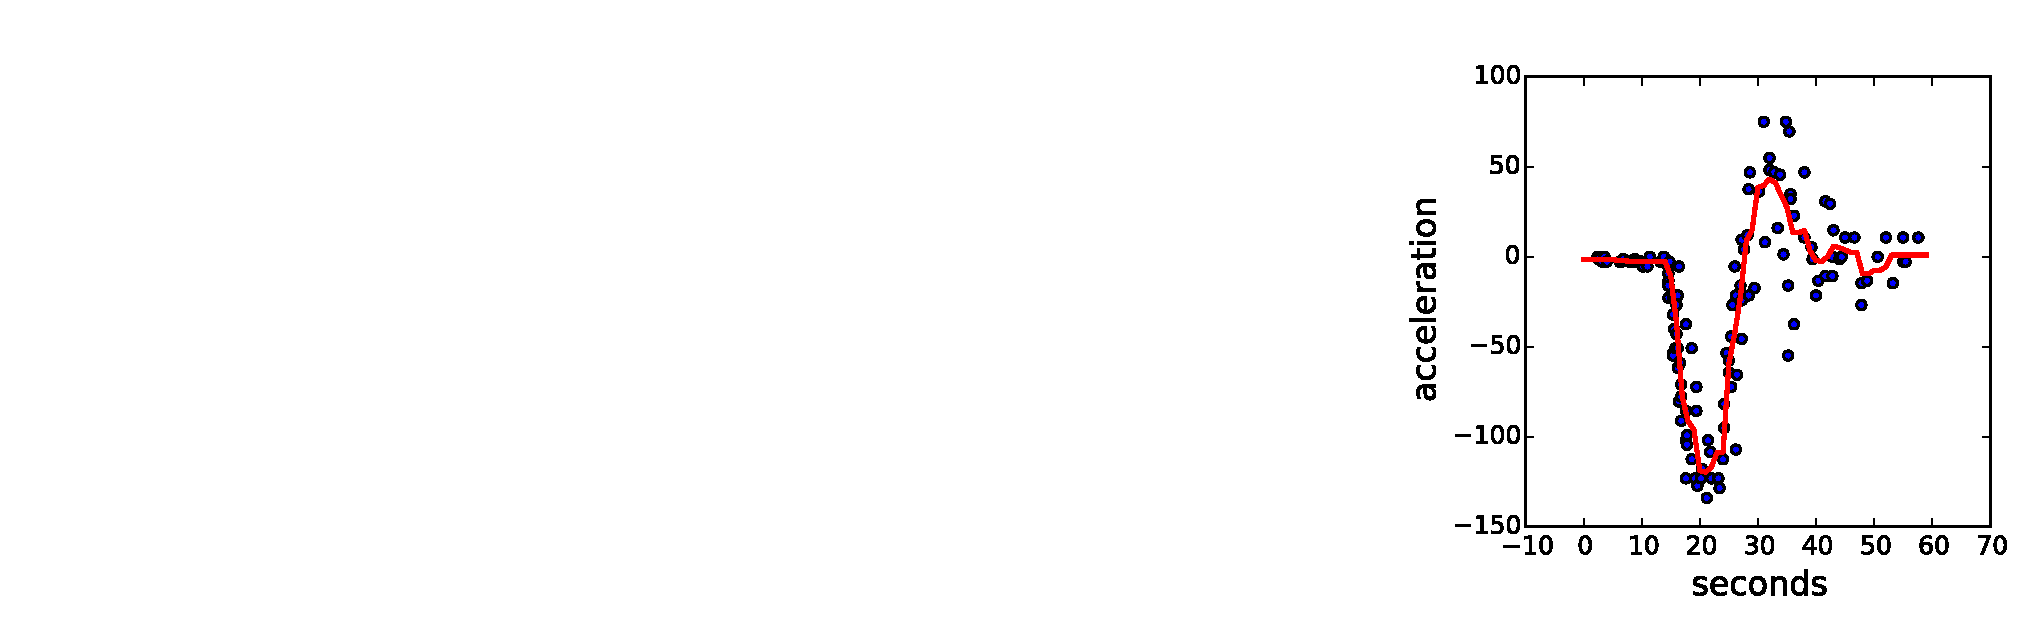
\includegraphics[height=1.75in]{../../bayesian-forest/graphs/MCbforest}   

\vskip .25cm{
Random Forest $\approx$ Bayesian forest $\approx$ posterior over CART fits.}

\vskip -.5cm

\end{frame}



\begin{frame}

{\bf Theoretical {\theme trunk} stability}

\vskip .5cm

Given forests as a posterior, 
we can start talking about {\it variance}.

\vskip .1cm

Consider the first-order approximation
\begin{eqnarray*}
\sigma^2(x,\bs{\theta}) \approx& \sigma^2(x,\boldsymbol{1}) + \nabla \sigma^2\big |_{\boldsymbol{\theta}=\mathbf{1}} (\boldsymbol{\theta} - \boldsymbol{1}) \\ &=  \frac{1}{n}\sum_i \theta_i \left[y_i - \bar{y}_i(x)\right]^2
\end{eqnarray*}
with $\bar y_i (x)$ the sample mean in $i$'s node when splitting on $x$.

\vskip .1cm
Based on this approx, we can say that for data at a given node, 
\begin{equation*}\theme
\mathrm{p}\left(\text{optimal split matches sample CART}\right) \gtrsim 1 - \frac{p}{\sqrt{n}} e^{-n},
\end{equation*}
with $p$ split locations and $n$ observations.  

% \vskip .5cm{\nv Things are pretty stable, until they aren't: as the tree grows,  node sizes get smaller and chance of a non-optimal split multiplies.}

\end{frame}

\begin{frame}

{\bf California Housing Data}


\vskip .5cm

20k observations on median home prices in zip codes.

\vskip .5cm

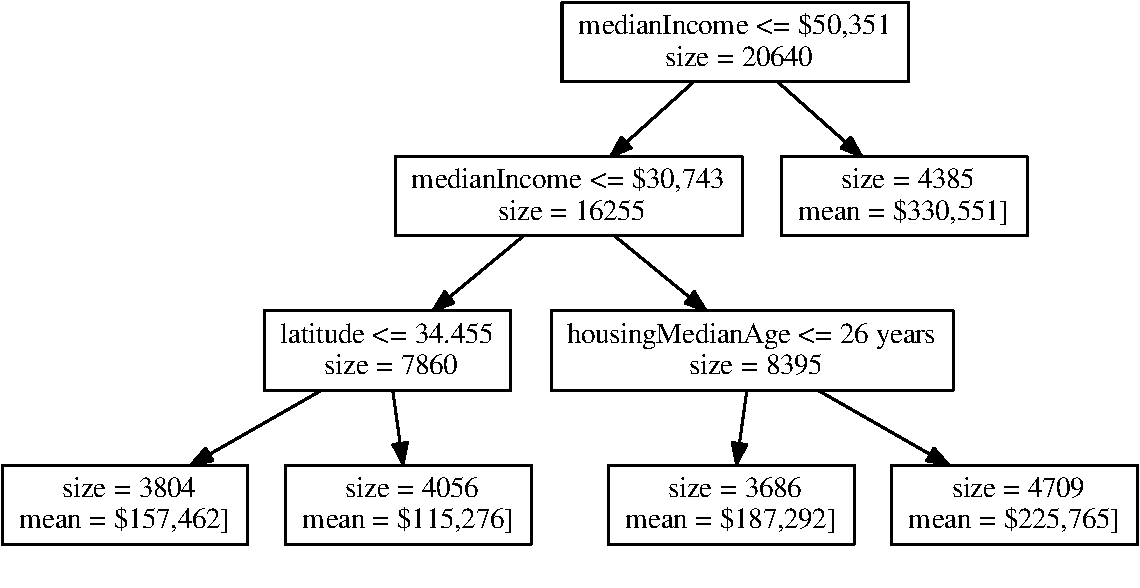
\includegraphics[width=\textwidth]{../../bayesian-forest/graphs/ca_trunk}

\vskip .5cm
\hfill Above is the trunk you get setting min-leaf-size of 3500.

\end{frame}

\begin{frame}

\begin{columns}

\begin{column}{2.15in}
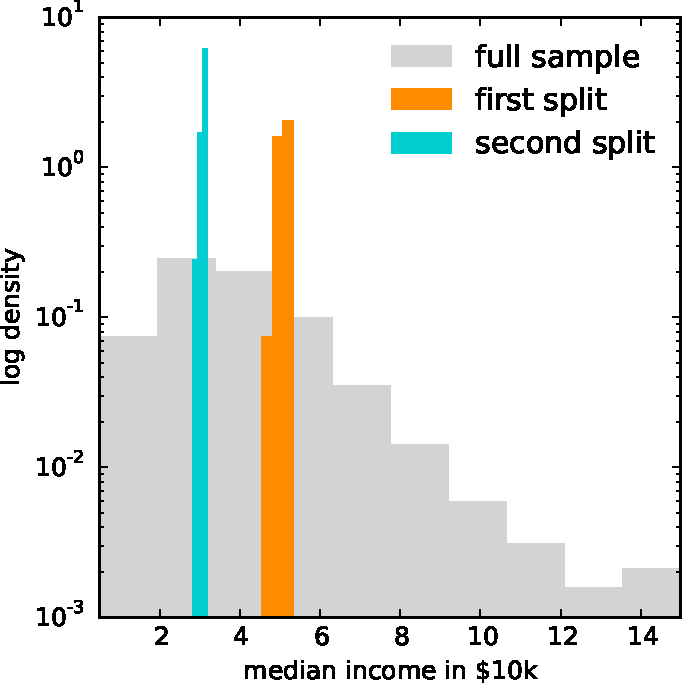
\includegraphics[width=2.5in]{../../bayesian-forest/graphs/ca_splits}
\end{column}

\begin{column}{2in}
\begin{itemize}
\item sample tree occurs 62\% \\of the time.  
\vskip .5cm
\item 90\% of  trees split on income twice, \\and then latitude. 

\vskip .5cm
\item 100\% of trees have 1st 2 splits on median income.  
\end{itemize}
\end{column}

\end{columns}


\vskip 1cm
~~~~Empirically and theoretically: trees are stable, at the trunk.
\vskip -1cm

\end{frame}

\begin{frame}

{\bf Empirical Bayesian Forests ({\theme EBF})}

\vskip .5cm
RFs are expensive.  Sub-sampling hurts bad.

\vskip .25cm
{Instead:}
\begin{itemize}
\item fit a single tree to a shallow {\nv trunk}.  
\item Map data to each {\nv branch}.  
\item Fit a full  forest on the smaller branch datasets.
\end{itemize}

\vskip .25cm
Empirical Bayes: fix plug-in estimates at high levels in a hierarchical model, focus effort at learning the hard bits.


\end{frame}

\begin{frame}


Since the trunks are all the same for each tree in a full forest,
our EBF looks nearly the same at a fraction of computational cost.

\begin{center}
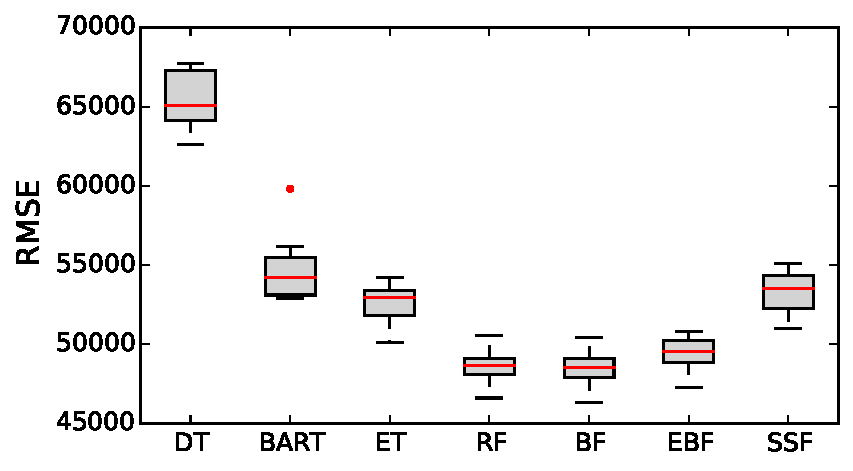
\includegraphics[width=.85\textwidth]{../../bayesian-forest/graphs/ca_rmse}
\end{center}

Here EBF and BF give nearly the same results.  {\it SSF does not.}


\end{frame}


\begin{frame}

{\bf EBFs work all over the place}

\vskip .5cm
\begin{minipage}{0.5\linewidth}
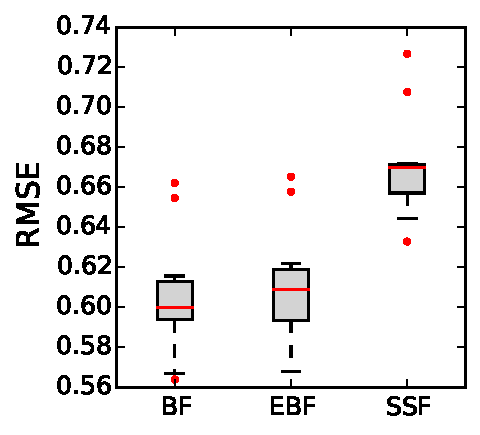
\includegraphics[width=\textwidth]{../graphs/wine}
\end{minipage}
~~
\begin{minipage}{0.4\linewidth}
{\footnotesize
\begin{tabular}{c c | l}
$\overline{\text{RMSE}}$  & \% WTB & \\
\cline{1-2}\rule{0pt}{3ex} 
0.5905 &  0.0 & BF \\
0.5953 &  0.8 & EBF \\
0.6607 & 11.9 & SSF \\
0.7648 & 29.5 & DT \\
\end{tabular}}
\end{minipage}

\vskip .5cm
\hfill Predicting wine rating from chemical profile

\end{frame}


\begin{frame}

{\bf EBFs work all over the place}

\vskip .5cm
\begin{minipage}{0.5\linewidth}
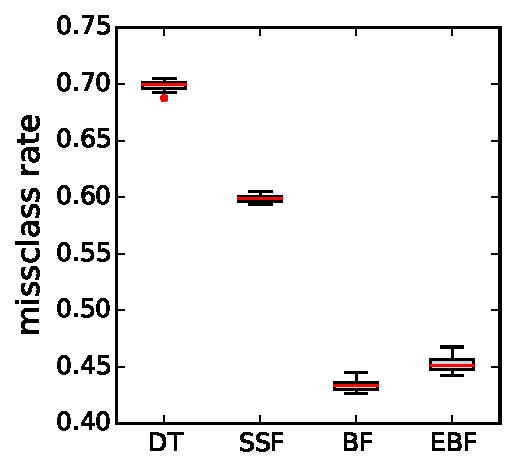
\includegraphics[width=\textwidth]{../graphs/beer}
\end{minipage}
~~
\begin{minipage}{0.4\linewidth}
{\footnotesize
\begin{tabular}{c c | l}
$\overline{\text{MCR}}$  & \% WTB & \\
\cline{1-2}\rule{0pt}{3ex} 
0.4341 &  0.0 & BF \\
0.4531 &  4.4 & EBF \\
0.5989 & 38.0 & SSF \\
0.6979 & 60.8 & DT \\
\end{tabular}}
\end{minipage}

\vskip .5cm
\hfill or beer choice from demographics

\end{frame}

\begin{frame}

{\bf Choosing the trunk depth}


\vskip .5cm
Distributed computing perspective: {\theme fix only as deep as you must!}

\vskip .1cm
How big is each machine? Make that your branch size.

\vskip .75cm
{\small
\begin{tabular}{c | c c c | c c c | c c c}
& \multicolumn{3}{l|}{CA housing} & \multicolumn{3}{l|}{Wine} &\multicolumn{3}{l}{Beer} \\
\cline{2-10} \rule{0pt}{3ex} 
\!\!\!\!\!\!{\it Min Leaf Size in $10^3$} & 6 & 3 & 1.5 & 2  & 1 & 0.5 & 20 & 10 & 5\\
\!\!\!\!\!\!{\it \% Worse Than Best} & \!1.6 & \!2.4 & \!4.3 & \!0.3 & \!0.8 & \!2.2 & \!1.0 & \!4.4 & \!7.6 
\end{tabular}}

\vskip .5cm
Still, open questions:  e.g., more trees vs shallower trunk?

\end{frame}

\begin{frame}

{\bf Catching Bad Buyer Experiences  at eBay}

\vskip .5cm
BBE: `not as described', delays, etc.

\vskip .5cm
~$\mathrm{p}(\text{BBE})$
is an input to search rankings.

\vskip .1cm ~~~~Best way to improve prediction is more data.  

\vskip .1cm ~~~~~~~~EBFs via Spark: more data in less time.

\vskip .5cm
On 12 million transactions,  EBF with 32 branches yields a\\ 1.3\% drop in misclassification over the SSF alternatives.  

\vskip .5cm
Putting it into production requires some careful engineering, \\but this really is a very simple algorithm.  {\theme Big gain, little pain.} 

\end{frame}

\begin{frame}

{\bf Heterogeneous Treatment Effects}

\vskip .5cm
Recall our earlier example: A/B experiment with user covariates $\bm{x}_i$.

\vskip .35cm
Athey\texttt{+}Imbens propose indexing user HTE by fitting CART to
\[
y^\star_i = y_i \frac{d_i - q}{q(1-q)} = \left\{
\begin{array}{cc}
y_i/(1-q) &\text{if~} d_i=0\\
y_i/q &\text{if~} d_i=1
\end{array}\right.
\]
where $q$ is the probability of treatment ($2/3$ in our example).

\vskip .35cm
This works because
\[
\ds{E}[y^\star_i | \bs{\upsilon}_i] = 
%q \upsilon_i(1)\frac{1 - q}{q(1-q)} - (1-q) \upsilon_i(0)\frac{q}{q(1-q)}
\upsilon_i(1)- \upsilon_i(0)
\]
where $\upsilon_i(d)$ is the potential outcome for user $i$ if $d_i = d$.\\  {\gr We only get to observe one of these: $y_i =
\upsilon_i(d_i)$.}

\end{frame}

\begin{frame}

We can apply the Bayesian bootstrap (i.e., fit a BF) to assess \\{\it posterior uncertainty} about these treatment-effect trees.

\vskip .15cm
e.g., sample depth-5 CART with min-leaf-size-$10^5$ after one week:
\begin{center}
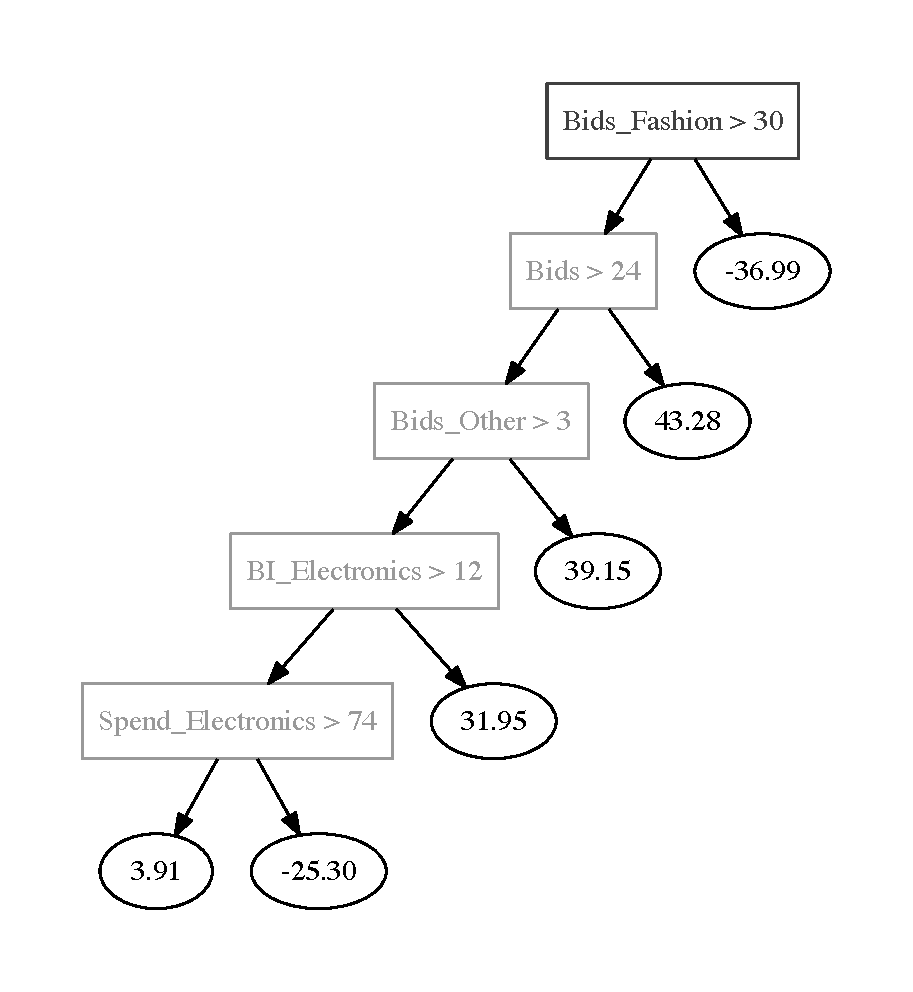
\includegraphics[width=.5\textwidth]{graphs/samptree_week1}
\end{center}
\hfill prob variable is node in tree: {\color{black!50} $\mr{p} <\tfrac{1}{3}$},
{\color{black!75}  $\mr{p} \in
\left[\tfrac{1}{3},\tfrac{1}{2}\right)$}, and {\color{DarkRed}  $\mr{p}
\geq \tfrac{1}{2}$}.
\end{frame}

\begin{frame}

After 5 weeks the tree is much more stable.
\begin{center}
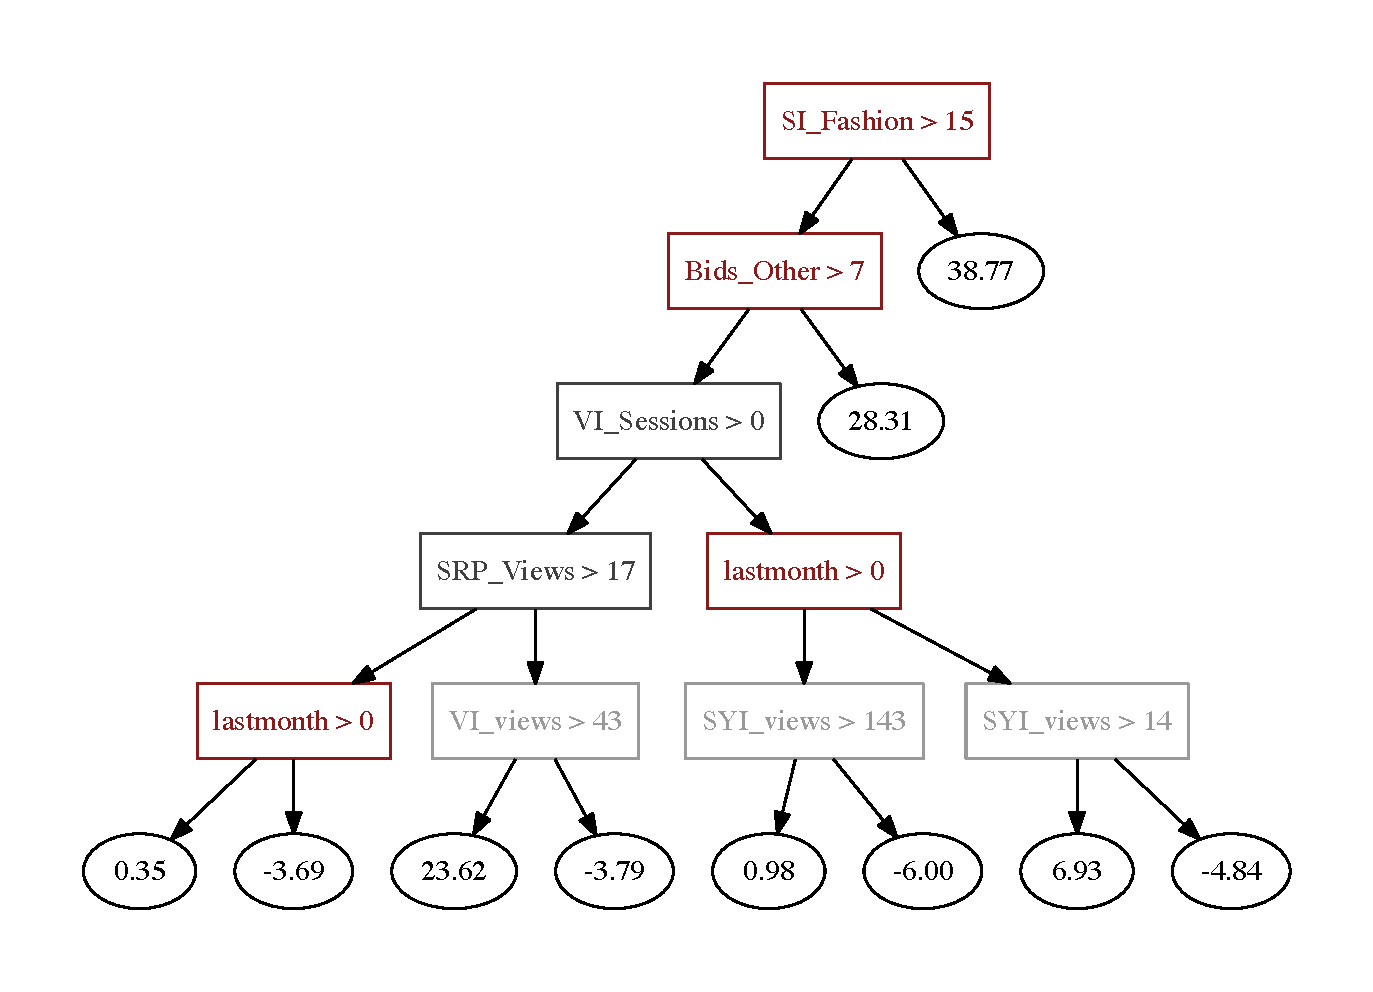
\includegraphics[width=.9\textwidth]{graphs/samptree_week5}
\end{center}

\end{frame}

\begin{frame}

We can quantify uncertainty about all sorts of structure.

\vskip .5cm
{\bf Posterior probability of CART splitting on variable}
\begin{center}
{\small
\begin{tabular}{l|ccccc}
\textbf{Week 5}& \multicolumn{5}{c}{\textit{depth in tree}}\\
 & $1$ & $\leq 2$ & $\leq 3$ & $\leq 4$ & $\leq 5$ \\
\hline
\rule{0pt}{1.25\normalbaselineskip}\textit{SI\,Fashion}
& .45 & .50 & .50 & .50 & .50\\
\textit{Bids\,Other} & .30 & .75 & .75 & .75 & .75\\
\textit{VI\,sessions} & .05 & .05 & .05 & .10 & .35\\
\textit{lastmonth} & .05 & .10 & .15 & .40 & .65\\
\textit{SRP\,views} & .00 & .10 & .15 & .25 & .40\\
\textit{VI\,views} & .00 & .00 & .10 & .20 & .25\\
\textit{SYI\,views} & .00 & .00 & .05 & .15 & .25
\end{tabular}}
\end{center}

\vskip .25cm
Simple scalable uncertainty quantification for complex algorithms.  

\end{frame}

\begin{frame}

\vskip .5cm
{\bf Big Data and distribution free BNP}

\vskip .25cm I think about BNP as a way to analyze (and improve) algorithms.  

Decouple  action/prediction from the full generative process model.

\vskip .75cm
{\bf Efficient Big Data analysis}

\vskip .25cm
To cut computation without hurting performance, we need to think about what portions of the `model' are {\theme hard} or {\nv easy} to learn.

\vskip .25cm
Once we figure this out,  we can use a little bit of the data to\\ learn the easy stuff and direct our full data at the hard stuff.

% \vskip .25cm
% I believe that this is the future for Big Data.


\vskip 1cm
\hfill \huge \theme \bf thanks!

\end{frame}





\end{document}






























